\documentclass[a4paper,10pt]{article}
%\usepackage[utf8x]{inputenc}

% Lay out packages
\usepackage[]{geometry}
\usepackage[utf8]{inputenc}
\usepackage{mathpazo}

\usepackage{amsmath}
\usepackage{graphicx}

% Dutch style of paragraph formatting, i.e. no indents. 
\setlength{\parskip}{1.3ex plus 0.2ex minus 0.2ex}
\setlength{\parindent}{0pt}

%opening
\title{Computer Vision Assignment 2: Feature Detection}
\author{Robrecht Jurriaans (5887380), Taco Cohen (6394590)}

\begin{document}

\maketitle



\section{Harris Corner Detection}
The Harris Corner Detector is based on the earlier work by Moravec \cite{Moravec1980} which defined corners as being points with low self-similarity. The similarity is taken as the sum of squared differences to larger overlapping patches around a point, see figure \ref{fig:harris}. This method is quite computationally expensive as it requires separate computation for each pixel in an image.

The Harris corner detection algorithm\cite{Harris1988} builds upon this idea but improves the efficiency by using a taylor-series approximation to the self-similarity surface.

\begin{figure}[ht]
\centering
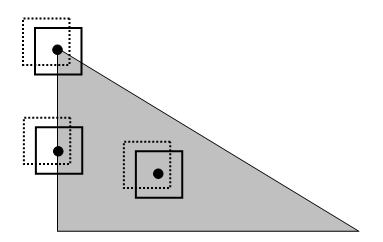
\includegraphics[width=0.7\textwidth]{img/cornermetric1}
\caption{A shifting window for a flat patch, an edge and a corner (Image taken from MathWorks)}
\label{fig:harris}
\end{figure}

If there is no edge or a corner within the window, the intensity values within the window will not change a lot. If the window contains an edge, moving the window along the edge will not result in any difference, but any movement along the perpendicular axis will result in a shift in intensity. For a corner, it does not matter which direction the window is shifted, as every window will be different.

By shifting the window in the $[u,v]$ direction we can compute the window-averaged change in intensity as follows:

\[E(u,v) = \sum_{x,y} E(x,y) [I(x+u,y+v) - I(x,y)]^2\]

where $W(x,y)$ represents the window function which can be $W(x,y)=1$ for all $x$ and $y$ within the window, or it can be a Gaussian function. $I(x+u, y+v)$ represents the shift in intensity and $I(x,y)$ represents the original intensity. For small values of $u$ and $v$ we can approximate this with a Taylor-series expansion and change the equation in:

\[E(u,v) \cong [u,v] M  \left[\begin{array}{c} u\\ v \end{array}\right] \]

where $M$ is the structure tensor, also known as the second moment matrix. It is defined as:

\[M = \sum_{x,y} W(x,y)  \begin{bmatrix}I^2_x & I_x I_y \\ I_x I_y &  I^2_y \end{bmatrix} \]

The structure tensor matrix $M$ can be used to determine the direction of the largest change by finding the eigenvalues $\lambda_1$ and $\lambda_2$ of $M$ where $\lambda_1$ represents the direction of the fastest change\footnote{Note that we assume the eigenvalues to be ordered from largest to smallest}, whilst $\lambda_2$ represents the direction of the slowest change. As can be seen in figure \ref{fig:isoresponse}.

\begin{figure}[ht]
\centering
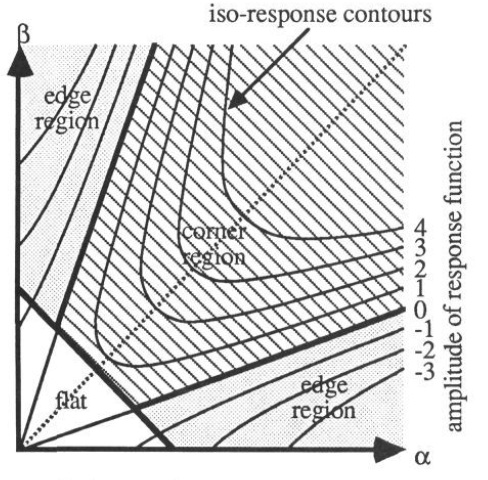
\includegraphics[width=0.7\textwidth]{img/isoresponse}
\caption{The iso-response surface for eigenvalues $\alpha$ and $\beta$ \cite{Harris1988}}
\label{fig:isoresponse}
\end{figure}

If both eigenvalues are low, then the change in intensity is small in all directions and thus the window is on a flat region. If one of the eigenvalues is larger than the other, the window is on an edge and when both eigenvalues are large then the change in intensity for every direction is large and the window is on a corner.

To avoid a costly calculation of the eigenvalues of $M$, it is possible to represent the cornerness $R$ by the determinant ($\lambda_1 \lambda_2$) and the trace ($\lambda_1 + \lambda_2$) of $M$ as follows:

\[R = \det( M ) - k(\operatorname{trace}( M ))^2\]

where $k$ is a small constant which is used to bias the detector towards corners or towards edges.
$k=0$ would focus solely on corners whereas $k=0.25$ would only return edges.
It is possible to avoid the use of this empirical constant $k$ by using Noble's measure of cornerness\cite{noble1989descriptions}:

\[M'_c = 2 \frac{\det( M )}{\operatorname{trace}( M ) + \epsilon}\]

\subsection{Implementation Details}
We have implemented the Harris corner detector in \verb+harris.m+.
Following Mikolajczyk et al.\cite{Mikolajczyk2004}, we use a constant $\gamma = 0.7$ to automatically determine the derivative scale from the given integration scale $\sigma$.
We use a morphological image operation (dilation) to determine local maxima in the cornerness image; see the code and its comments for further details.

\section{Harris-Laplace}
The basic Harris corner detector is not scale-invariant.
To gain scale invariance we implemented the Harris-Laplace detector from \cite{Mikolajczyk2004}.
Although there are a number of subtleties in the implementation of this detector (Mikolajczyk's original algorithm uses an iterative procedure to find the characteristic scales), we have implemented a simple variant as follows.
We first detect Harris corners at several scales, spaced appart by a factor of $1.4$.
Next, for each keypoint we look at the neighbouring scales if the scale-normalized Laplacian is at a scale-space extremum.
If it is, we keep the corner point (at the found scale), otherwise we reject it.
It is also possible to use an additional threshold on the value of the Laplacian.

Our implementation can be found in \verb+harris_laplace.m+.

\section{SIFT}
After finding corners with the Multi-scale Harris Corner Detection, SIFT descriptors are created for each of these corners.
We use the publicly available \verb+vl_feat+ SIFT implementation, which must be installed to run our code.
We only use the SIFT \emph{descriptor} and not the keypoint detector from \verb+vl_feat+.
We do use the \verb+vl_ubcmatch+ function for descriptor matching, but we have written code for this too; see the commented code block in \verb+findMatches.m+.


\section{Mosaic}
To evaluate the matches, we estimate the homography matrix $H$ using RANSAC by fitting the linear least squares solution to a set of matching points $p_1$ and $p_2$. All point pairs are then evaluated if they are within a given threshold $t$ by $((H p_1)-p_2)^2 < t$ and if so, they are classified as inliers for the estimated model. A new model is fitted on all inliers and a final score is calculated for the model. After $n$ iterations the best model is returned and used to transform the image to the new image plane. 

\begin{figure}[h!t]
\centering
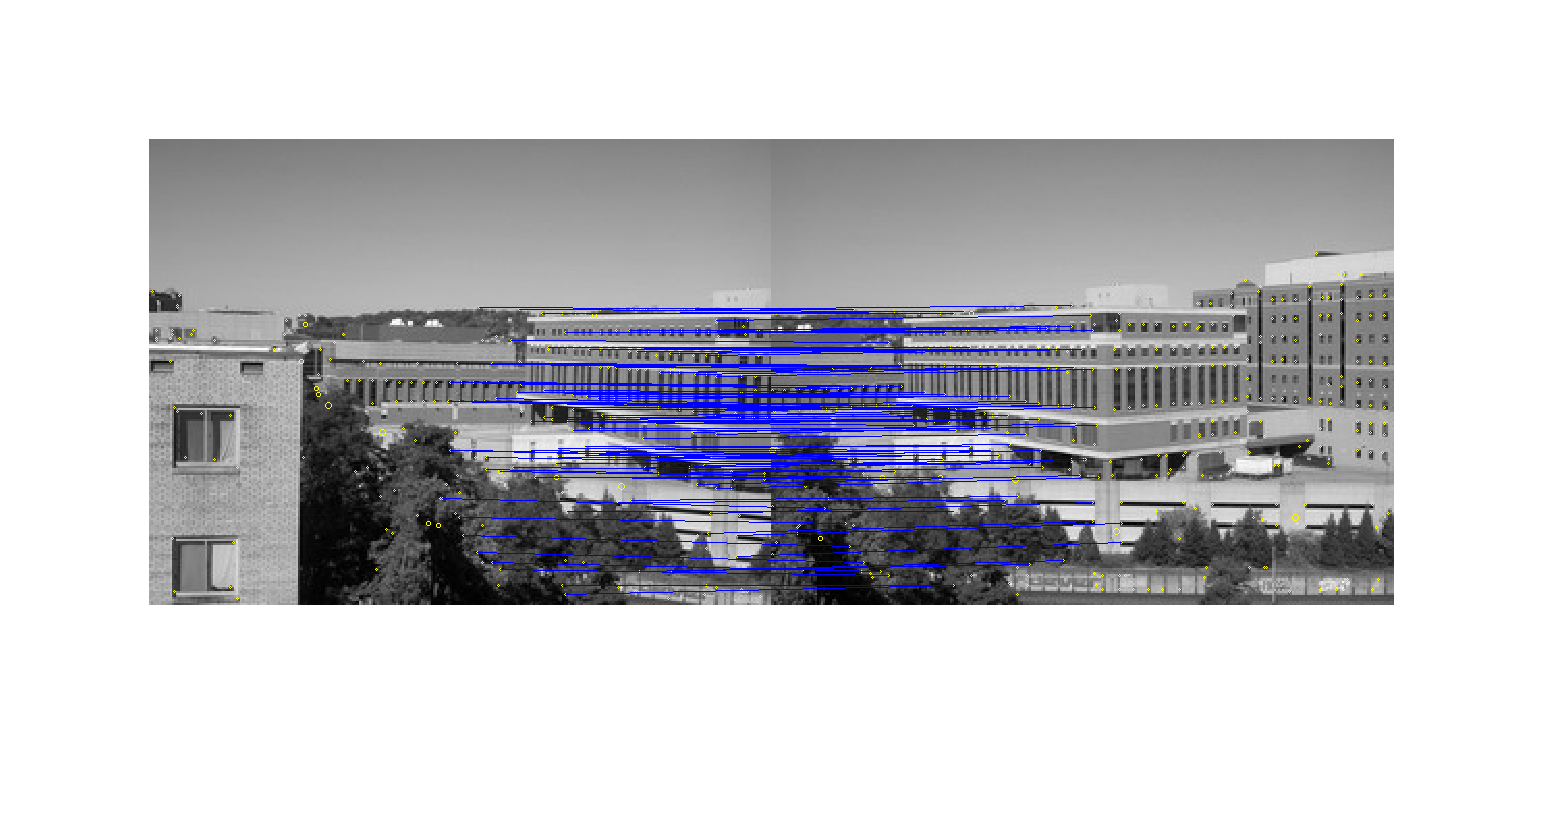
\includegraphics[width=0.8\textwidth]{img/mosaicmatch}
\caption{Matches found between sift descriptors of harris corners in two images from same optical centre}
\label{fig:mosaicmatch}
\end{figure}

In the landscape images, there is a large translation between both camera positions in the $z$-direction. Therefore, mosaicing these images is very difficult as there is no projective transformation that can account for this. However, by using images, as seen in figure \ref{fig:mosaicmatch}, that are taken from the same optical centre it becomes possible to stitch the images together to form a mosaic, as can be seen in figure \ref{fig:mosaic}.

\begin{figure}[h!t]
\centering
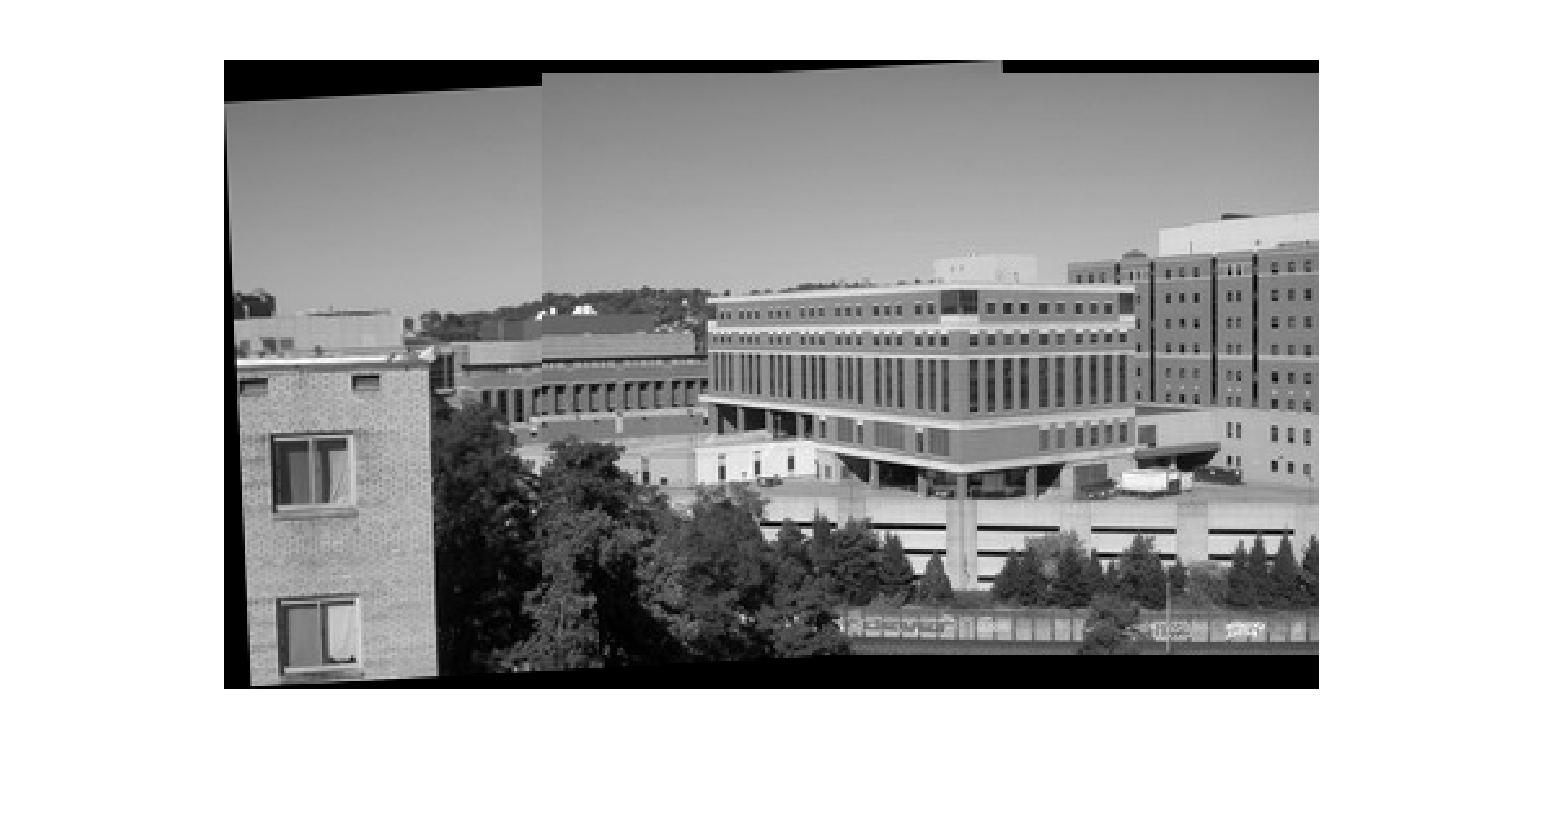
\includegraphics[width=0.8\textwidth]{img/mosaic}
\caption{Image mosaic made by estimating homography using RANSAC}
\label{fig:mosaic}
\end{figure}

\section{DoG versus LoG}
A fast alternative to the scale-normalized Laplacian is the Difference of Gaussians (DoG).
We implemented this the usual way, by calculating the Gaussian blurred images at several scales, and then creating difference maps of subsequent levels.
The results are qualitatively very similar to the LoG results, see figure \ref{fig:logdog}.

DoG can be used in the \verb+harris_laplace+ function by passing 'DoG' for the mode parameter.
We did some quick tests, and on our system the \verb+harris_laplace+ with 'DoG' takes about $0.9$ seconds to execute, whereas with 'LoG' it takes about $1.1$ seconds.
Of course, both versions could be optimized further.
In terms of matching performance, the two approaches appear to have a similar accuracy, but this is a subjective judgement.
A rigorous repeatability study is beyond the scope of this report.

\begin{figure}[h!t]
\centering
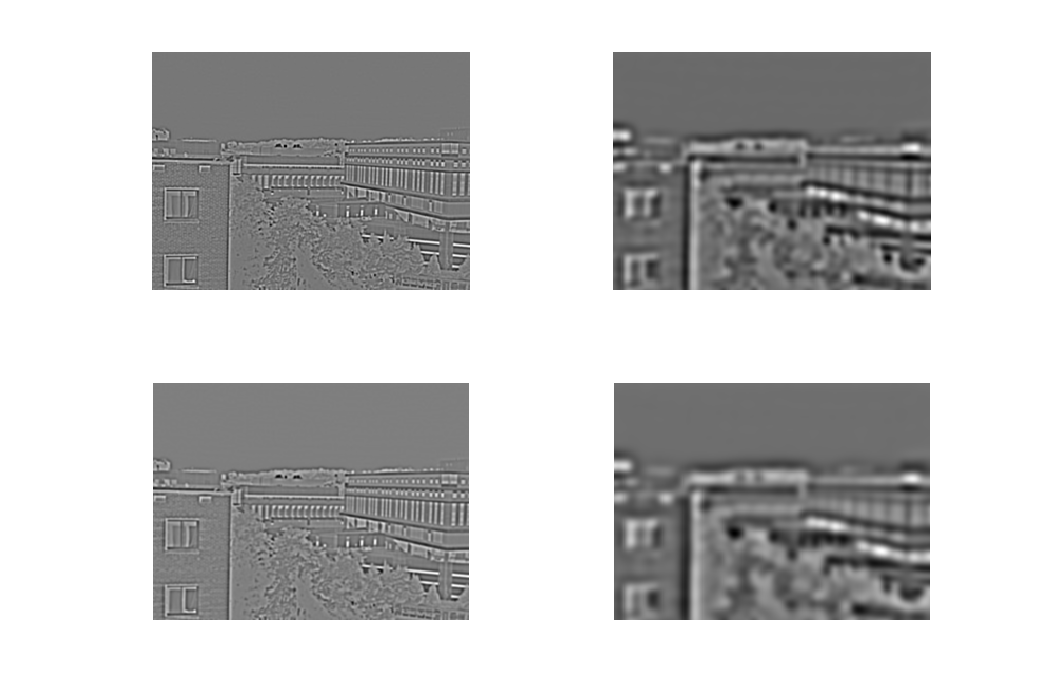
\includegraphics[width=0.95\textwidth]{img/LOG_DOG}
\caption{LoG (top) versus DoG (bottom) at scales $\sigma = 1$ and $\sigma = 4$.}
\label{fig:logdog}
\end{figure}

\bibliographystyle{plain}
\bibliography{references}

\clearpage
\appendix
\section{Running the code}
The file \verb|master.m| can be run to load in the two landscape images. It runs findmatches with a very high threshold (250) because we then use Lowe's method to reject any matches where the ratio of distance in descriptors is above $0.8$ for the closest descriptor and the second closest. \verb|findMatches.m| uses \verb|harris_laplace.m| to find the corners using either Laplacians or DoG. The Harris detector also has a threshold which we set at $0.01*\max(R)$, but which can be set higher to reject more features or lower to allow for more features. This setting is domain dependent and thus we will wait for the next assignments to further tweak this threshold. The findMatches function also shows both images next to each other with scatter plots to show the features. However, this will cause the program to crash if the used images are not equal in size.

In the file \verb|ransacmaster.m| the same code as above is ran, but this time the matches are used to estimate a homography matrix to make a mosaic image. Ransac is ran for 100 iterations and can be further tweaked with the threshold for inliers and the minimum required inliers for a model. Again, the landscape images are not fit to be used to stitch the images due to the difference in optical centre.



\end{document}
